\documentclass{frontiersSCNS}
\usepackage{url,hyperref,lineno,microtype,subcaption}
\usepackage[onehalfspacing]{setspace}
\usepackage{float}


\linenumbers

\usepackage[utf8]{inputenc}
\floatplacement{figure}{H}

\def\keyFont{\fontsize{8}{11}\helveticabold }
\def\firstAuthorLast{Villaseñor-Derbez {et~al.}}
\def\Authors{Juan Carlos Villaseñor-Derbez\(^{1,*}\), Eréndira
Aceves-Bueno\(^{1,*}\), Álvin Suarez-Castillo\(^{2}\), Stuart
Fulton\(^{2}\), Jorge Torre\(^{2}\)}
% Affiliations should be keyed to the author's name with superscript numbers and be listed as follows: Laboratory, Institute, Department, Organization, City, State abbreviation (USA, Canada, Australia), and Country (without detailed address information such as city zip codes or street names).
% If one of the authors has a change of address, list the new address below the correspondence details using a superscript symbol and use the same symbol to indicate the author in the author list.
\def\Address{\(^{1}\)Bren School of Environmental Science and Management, University
of California, Santa Barbara, Santa Barbara, CA,
USA\newline \(^{2}\)Comunidad y Biodiversidad A.C., Guaymas, Mexico}
% The Corresponding Author should be marked with an asterisk
% Provide the exact contact address (this time including street name and city zip code) and email of the corresponding author
\def\corrAuthor{Juan Carlos Villaseñor-Derbez, Bren Hall, University of California,
Santa Barbara, Santa Barbara, CA, 93106}

\def\corrEmail{\href{mailto:jvillasenor@bren.ucsb.edu}{\nolinkurl{jvillasenor@bren.ucsb.edu}}}

\usepackage{amsthm}
\newtheorem{theorem}{Theorem}[section]
\newtheorem{lemma}{Lemma}[section]
\theoremstyle{definition}
\newtheorem{definition}{Definition}[section]
\newtheorem{corollary}{Corollary}[section]
\newtheorem{proposition}{Proposition}[section]
\theoremstyle{definition}
\newtheorem{example}{Example}[section]
\theoremstyle{definition}
\newtheorem{exercise}{Exercise}[section]
\theoremstyle{remark}
\newtheorem*{remark}{Remark}
\newtheorem*{solution}{Solution}
\begin{document}
\onecolumn
\firstpage{1}

\title[Marine reserve effectiveness]{Enabling conditions for effective community-based marine reserves in
small-scale fisheries} 

\author[\firstAuthorLast ]{\Authors} %This field will be automatically populated
\address{} %This field will be automatically populated
\correspondance{} %This field will be automatically populated

\extraAuth{}

\maketitle



\begin{abstract}

Coastal marine ecosystems provide livelihoods for small-scale fishers
and coastal communities around the world. However, overfishing and
unsustainable fishing practices threaten the marine environment and
jeopardize the wellbeing of coastal communities. A common approach to
protect the environment and recover overexploited stocks is to implement
no-take marine reserves (areas where all extractive activities are
off-limits). In small-scale fisheries, these are sometimes implemented
as community-based reserves, where a group of fishers collectively agree
to close an area to fishing. While we know that reductions in fishing
effort are followed by a series of ecological benefits (increased
biomass, abundance, and species diversity), we do not fully understand
how environmental and governance dynamics influence the conservation and
fisheries benefits of community-based marine reserves. In this work, we
evaluate the ecological outcomes of four reserves established by three
coastal communities in temperate and tropical ecosystems of Mexico. By
combining causal inference techniques with an operationalization of the
social-ecological systems framework, we identify the environmental and
social conditions that enable reserve effectiveness. Our results show a
strong interaction between environmental variation and community
organization, which influences reserve effectiveness. For example, the
most effective reserve had strong governance structures accompanied with
low environmental variability. Thus, even when a community is well
organized (and reserves are well enforced), environmental variation can
hinder the benefits of a reserve, and vice versa. Our results are
particularly relevant under present changing climate conditions, as they
can better inform management and decision making.




\medskip
\tiny
 \keyFont{ \section{Keywords:} Marine Protected Areas, Marine Conservation, Small-Scale Fisheries,
Citizen Science, Mexico, Social-Ecological Systems}



\end{abstract}


\textbf{Last\_update}: 2018-04-10

\clearpage

\section{Introduction}\label{introduction}

Marine ecosystems around the world sustain significant impacts due to
overfishing and unsustainable fishing practices
\citep{halpern_2008-dK,worm_2006-IB,pauly_2005-qV}. A common approach to
manage the spatial distribution of fishing effort and recover stocks is
through the implementation of marine reserves (\emph{i.e.} areas where
all fishing activities are off--limits; MRs)
\citep{afflerbach_2014-HP,krueck_2017-J1,sala_2017-69}.

Marine reserve science has largely focused on understanding the
ecological effects of these areas, which include increased biomass,
richness, and densities of organisms within the protected regions
\citep{lester_2009-Ks,giakoumi_2017-V2,sala_2017-69}, climate change
mitigation \citep{roberts_2017-J9}, and protection from environmental
variability \citep{micheli_2012-EU}. However, there is considerably less
literature focusing on the relationship between socioeconomic and
governance structures and their relationship to ecological effectiveness
\citep{halpern_2013,lpezangarita_2014,mascia_2017-m_} or benefits to
fisheries \citep{krueck_2017-J1}; evaluations of marine reserves rarely
provide a holistic view of the social-ecological system
\citep{lpezangarita_2014}. Here, we combine causal inference techniques
\citep{depalma_2018} and the social-ecological systems framework
\citep{ostrom_2009-hg} to provide a comprehensive ecological and
socioeconomic evaluation of four community-based marine reserves in
three coastal communities in Mexico.

Marine Reserves in Mexico have been commonly implemented as ``core
zones'' within Biosphere Reserves that are administered by the National
Commission of Protected Areas (\emph{Comisión Nacional de Áreas Marinas
Protegidas}, CONANP). While CONANP has made efforts to have a
participatory process, the implementation of these zones is still
characterized by top--down approaches. This motivated Civil Society
Organizations (CSOs) to work with coastal communities to implement
community--based marine reserves \citep{uribe_2010-u2}, which are
usually established within a Territorial Use Rights for Fisheries
(TURFs); thus making them TURF--reserves \citep{afflerbach_2014-HP}.
This bottom--up approach allows fishers to design their own reserves,
which increases compliance and self--enforcement
\citep{gelcich_2015-Gw,espinosaromero_2014-PY,beger_2004-Y8}. However,
these reserves still lack legal recognition, making them vulnerable to
poaching. In 2014, a new norm \citep{nom} allowed fishers to request the
legal recognition of a community--based reserve under the name of
``Fishing Refugia'' (\emph{Zona de Refugio Pesquero}, FR). This new norm
thus combines bottom--up approaches to design marine reserves, along
with a legal recognition of the management intervention. Since then,
\emph{39} FR have been implemented along the Pacific, Gulf of
California, and Mexican Caribbean coastlines, but no formal evaluation
of their effectiveness has taken place.

While there are ecological factors defining the success of a MR
(\emph{i.e.} habitat representation, initial state of protection,
connectivity to other protected areas), their effectiveness also depends
on the socioeconomic and governance settings under which they are
implemented. Literature shows that many non-ecological characteristics
can play an equally important role in the effectiveness of MRs. For
example, age of a reserve (\emph{i.e.} time since its implementation),
size, and habitat contained were key to the effectiveness of MRs in
Palau \citep{friedlander_2017-oI}. In the Mediterranean,
\citet{difranco_2016-Xw} identify that surveillance and enforcement,
presence of a management plan, and involvement of fishers in management
and decision--making along with promotion of sustainable fishing
practices were the key factors that increased stock health and income to
fishers. At a global level, \citet{edgar_2014-UO} indicate that
enforcement, age, size, and isolation were important factors determining
effectiveness of the reserves.

The objective of this work is twofold: i) Provide the first evaluation
of community--based marine reserves in Mexico, and ii) provide a
comprehensive evaluation of the social--ecological system to identify
how socioeconomic and governance characteristics relate to ecological
effectiveness. With the purpose of providing a holistic evaluation, we
combine ecological, socioeconomic, and governance indicators. We use
causal inference techniques to provide a measurement of the effect of
the management intervention, and combine it with the social--ecological
systems framework \citep{ostrom_2009-hg}.

\section{Materials and Methods}\label{materials-and-methods}

\subsection{Study area}\label{study-area}

We focus our evaluation in three coastal communities from the Pacific
coast of Baja California (n = 1) and the Mesoamerican Reef System (n =
2; Fig \ref{fig:map}). Isla Natividad (IN) lies west of the Baja
California Peninsula (Fig \ref{fig:map}B), where kelp forests
(\emph{Macrocystis pyrifera}) and rocky reefs are the predominant
habitats. The island is home to a fishing cooperative (\emph{Sociedad
Cooperative de Producción Pesquera Buzos y Pescadores de la Baja
California SCL}), that holds a TURF for spiny lobster (\emph{Panulirus
interruptus}). However, other resources like finfish (yellow-tail jack,
\emph{Seriola lalandi}), sea cucumber (\emph{Parastichopus
parvimensis}), red sea urchin (\emph{Mesocentrotus franciscanus}), snail
(\emph{Megastraea turbanica} y \emph{M. undosa}), and abalone
(\emph{Haliotis spp}, until 2010) are also important sources of income.
In 2006, the community decided to implement two community--based marine
reserves within their fishing grounds, seeking to recover depleted
stocks of invertebrate species (mainly lobster and abalone). Until
today, these reserves are yet to be legally recognized as Fishing
Refugia.

The other two communities are Maria Elena (ME; Fig \ref{fig:map}C) and
Punta Herrero (PH; Fig \ref{fig:map}D) in the Yucatan Peninsula, where
coral reefs and mangroves are the representative coastal ecosystems. ME
is a fishing camp --visited intermittently during the fishing season--
belonging to the Cozumel fishing cooperative. PH is home to the ``José
María Azcorra'' fishing cooperative. The main source of income to both
communities is the Caribbean spiny lobster fishery (\emph{Panulirus
argus}), which is carried out within their respective TURFs. These
communities also target finfish in the off season, mainly snappers
(Lutjanidae) and groupers (Serranidae). ME established eight marine
reserves in 2012, and PH established four marine reserves in 2013. All
these reserves are legally recognized as Fishing Refugia.

\subsection{Data collection}\label{data-collection}

To perform the evaluation of these reserves we use thee sources of
information. Ecological data come from the annual ecological monitoring
of reserve and control areas, carried out by members from each community
and personnel from the Mexican CSO ``Comunidad y Biodiversidad''
(\href{www.cobi.org.mx}{COBI}). These monitorings record richness and
abundances of fish and invertebrate species in the reserves and control
sites. For fish census, size structures are also collected to derive
biomass. We define control sites as regions with habitat characteristics
similar to the corresponding reserves, and that presumably had the same
probability of being selected as reserves during the design phase. From
all the reserves in these three communities, we use the ones that have
data for reserve and control sites before and after the implementation
of the reserve. This provides us with a Before-After-Control-Impact
(\emph{i.e.} BACI) design that allows us to capture and control for
temporal and spatial dynamics \citep{depalma_2018,ferraro_2006-oW}. BACI
designs and causal inference techniques have proven effective to
evaluate marine reserves, as they allow us to causally attribute
observed changes to the intervention
\citep{moland_2013-VP,Villasenor-Derbez_2018}. All reserves were
surveyed annually from at least one year before implementation until
2016. Table \ref{table:com_sum} shows a summary of the number of
reserves, year of implementation, and number of transects for each
reserve.

\begin{figure}
\centering
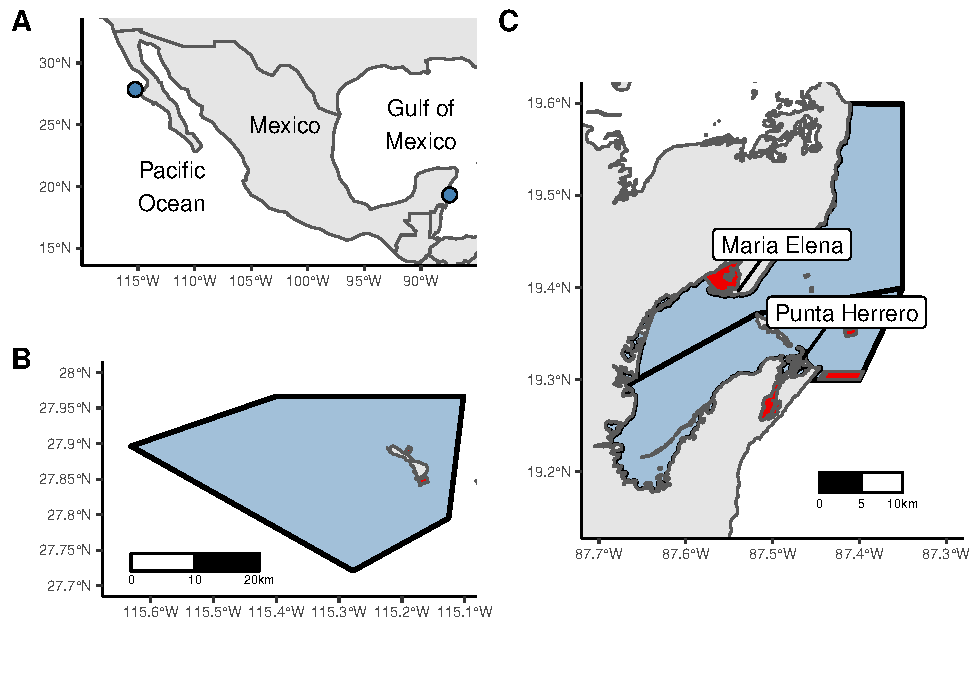
\includegraphics{Villasenor-Derbez_files/figure-latex/unnamed-chunk-1-1.pdf}
\caption{\label{fig:unnamed-chunk-1}\label{fig:map}Location of the three
coastal communities studied (A). Isla Natividad (B) is located off the
Baja California Peninsula, Maria Elena (C) and Punta Herrero (D) are
located in the yucatan Peninsula.}
\end{figure}

\begin{table}

\caption{\label{tab:unnamed-chunk-2}\label{table:com_sum} Summary of commuity--based marine reserves by community. Imp = Year of implementation, Start = Year of first sampling, number of fish transects in control (Cf) and reserve (Rf) sites, and number of invertebrate transects in Control (Ci) and Reserve (Ri) sites.}
\centering
\begin{tabular}[t]{l|l|r|r|r|r|r|r}
\hline
Community & Reserve - Control & Imp & Start & Cf & Rf & Ci & Ri\\
\hline
Isla Natividad & La Plana / Las Cuevas - La Dulce / Babencho & 2006 & 2006 & 400 & 241 & 415 & 244\\
\hline
Maria Elena & Cabezo - Cabezo (Control) & 2012 & 2012 & 44 & 45 & 27 & 21\\
\hline
Punta Herrero & El Faro - El Faro (Control) & 2013 & 2013 & 39 & 40 & 24 & 32\\
\hline
Punta Herrero & Manchon - Manchon (Control) & 2013 & 2012 & 43 & 45 & 27 & 41\\
\hline
\end{tabular}
\end{table}

Socioeconomic data come from landing receipts reported to the National
Commission for Aquaculture and Fisheries (\emph{Comisión Nacional de
Acuacultura y Pesca}; CONAPESCA). Data contain monthly lobster landings
(Kg) and value (MXP) from 2000 to 2014. This information was aggregated
by year, and economic values were adjusted by the Consumer Price Index
\citep{oecd_2017-VV} via Eq \ref{eqn:cpi}.

\begin{equation}
I_t = RI_t\times\frac{CPI_t}{CPI_T}
\label{eqn:cpi}
\end{equation}

Where \(I_t\) represents the adjusted income for year \(t\) as the
product between the reported income for that year and the ratio between
the consumer price index in that year (\(CPI_t\)) to the most recent
year's consumer price index (\(CPI_T\)).

Governance data were collected at the community-level. The information
was compiled by combining key informants and the authors; experience and
knowledge of the communities to collect the necessary information. These
data contain information on the ecological system where the fishing
activities develop, as well as the governance structures present in the
cooperative. We also gathered information on the resource unit
(\emph{i.e.} lobsters) and the relevant actors present in each community
\citep{leslie_2015-na}.

\subsection{Data analysis}\label{data-analysis}

Following a framework that relates reserve objectives to performance
indicators \citep{Villasenor-Derbez_2018}, we use five biological and
two socioeconomic indicators to evaluate these marine reserves Table
\ref{table:indicators}. We also use a set of governance indicators to
analyze the governance structures of each cooperative
\citep{leslie_2015-na}. The indicators (Table \ref{table:gov_ind}) focus
on the resource system (four indicators), governance system (seven
indicators), resource units (three indicators) and actors (three
indicators).

\begin{table}[H]

\caption{\label{tab:unnamed-chunk-3}\label{table:indicators}List of indicators used to evaluate the effectiveness of marine reserves, grouped by category.}
\centering
\begin{tabular}[t]{l|l}
\hline
Category & Indicador\\
\hline
Biological & Abundance\\
\hline
 & Richness\\
\hline
 & Shannon's diversity index\\
\hline
 & Biomass\\
\hline
 & Abundance of target species (lobsters)\\
\hline
Socioeconomic & Income from target species\\
\hline
 & Landings from target species\\
\hline
\end{tabular}
\end{table}

\begin{table}

\caption{\label{tab:unnamed-chunk-4}\label{table:gov_ind}Indicators used for the operationalization of the SES framework \citep{leslie_2015-na}}
\centering
\begin{tabular}[t]{>{\raggedright\arraybackslash}p{10em}|>{\raggedright\arraybackslash}p{8em}|>{\raggedright\arraybackslash}p{8em}|>{\raggedright\arraybackslash}p{8em}}
\hline
Indicator & Isla Natividad & Maria Elena & Punta Herrero\\
\hline
\textbf{Resource systems (RS)} & \textbf{} & \textbf{}\\
\hline
TURF presence & Yes & Yes & Yes\\
\hline
Type of ecosystem & Kelp Forest / Rocky Reefs & Coral Reef & Coral Reef\\
\hline
Intensity of environmental Disturbance & El nino event & Hurricanes & Hurricanes\\
\hline
Location & Island & Coastal & Coastal\\
\hline
\textbf{Governance systems (GS)} & \textbf{} & \textbf{}\\
\hline
Fishing cooperative & Yes & Yes & Yes\\
\hline
Involved actors & COBI, Stanford, REBIVI & Alianza Kanan Kay, COBI, CONANP, Coop, CONAPESCA, Oceanus, FCyRH, FHMM, & Alianza Kanan Kay, COBI, CONANP, Coop, CONAPESCA, Oceanus, FCyRH, FHMM,\\
\hline
Presence of an inter-cooperative structure & Fedecoop & Non & Non\\
\hline
Fishing Regulations & Size limits, seasonal closures, quotas & Size limits, seasonal closures & Size limits, seasonal closures\\
\hline
Enforcement technology & Boats & Boats & Land enforcement\\
\hline
MR enforcement &  &  & \\
\hline
Cooperative regulations &  &  & \\
\hline
\textbf{Resource Units (RU)} & \textbf{} & \textbf{}\\
\hline
Adult targeted species mobility & 1km & 30km & 30km\\
\hline
Targeted species longevity (years) &  &  & \\
\hline
Price of targeted species &  &  & \\
\hline
\textbf{Actors (A)} & \textbf{} & \textbf{}\\
\hline
Leadership &  &  & \\
\hline
Level of illegal fishing & 1 & 1 & 3\\
\hline
Presence of alternative livelihoods &  &  & \\
\hline
\end{tabular}
\end{table}

Biological indicators are analyzed with a difference--in--differences
analysis (Eq \ref{eqn:reg_bio}), which allows us to estimate the effect
that the reserve has on the biological indicators by comparing trends
across time and treatments
\citep{moland_2013-VP,Villasenor-Derbez_2018}. The analysis is performed
with generalized linear models of the form:

\begin{equation}
I_i = \alpha_{i} + \gamma_{it} Year_t + \beta Zone_i + \lambda_{it} Year_t\times Zone_i + \sigma_jSpp_j + \epsilon
\label{eqn:reg_bio}
\end{equation}

Where year--fixed effects are represented by \(\gamma_{it} Year_t\), and
\(\beta Zone_i\) captures the difference between reserve (\(Zone = 1\))
and control (\(Zone = 0\)) sites. The interaction term
\(\lambda_{it} Year_t\times Zone_i\) represents represent the mean
change in the indicator inside the reserve, for year \(t\), with respect
to the first year of evaluation in the control site (See Table
\ref{table:com_sum}). When evaluating biomass and abundances, we include
species--fixed effects (\(\sigma_j\)). For abundances and richness
(\emph{i.e.} count data) the model is estimated with a quasipoisson
error distribution.

Socioeconomic indicators are evaluated with a similar approach (Eq
\ref{eqn:soc_reg}), where landings and income before and after the
implementation of the reserve are compared:

\begin{equation}
I_i = \beta_0 + \beta_1Post
\label{eqn:soc_reg}
\end{equation}

This approach does not allow for a causal attribution of the observed
changes to the reserve, but still allows us to draw important
information that can inform our conclusions. For both approaches, model
coefficients are estimated via ordinary least--squares and
heteroskedastic--robust standard errors \citep{zeileis_2004-7n}.

\section{Results}\label{results}

Our methodological approach with biological indicators allows us to make
a causal link between the implementation of marine reserves and the
observed trends by accounting for temporal and spatial dynamics
\citep{depalma_2018}. The effect of the reserve is captured by the
\(\lambda_t\) coefficient, and represents the difference observed
between the control site before the implementation of the reserve and
the reserve site at time \(t\) after controlling for other time and
space variations (\emph{i.e.} \(\gamma_t\) and \(\beta\) respectively).
Here we present the effect that marine reserves had on each of the
biological indicators for each coastal community, along with the trends
in socioeconomic indicators of lobster catches and revenues. We also
provide an overview of the state of the socioeconomic and governance
settings of each community, and discuss how these dimensions might be
intertwined with each other.

\subsection{Biological}\label{biological}

Effect sizes for biological indicators are shown in Figure
\ref{fig:indicators}, and Figure \ref{fig:res_com} shows the summarized
biological effects by community. Isla Natividad shows inconsistent
effects across data sources (\emph{i.e.} fish vs.~invertebrates). For
example, the reserve had a small effect on fish abundances (Fig
\ref{fig:indicators}A), where only year 2010 showed significant effect
sizes in fish abundances (\(p<0.05\)) and all other years oscillated
above and under zero (\(p > 0.05\)). However, invertebrate abundances
(Fig \ref{fig:indicators}B) presented a positive trend relative to the
control site before implementation (\(p < 0.05\)) for all but 1 year
(2008). Maria Elena and Punta Herrero showed no significant increase in
fish and invertebrate abundances (\(p< 0.05\)), except for invertebrates
in Punta Herrero for 2014 --right after the implementation of the
reserves-- which showed a significant increase (\emph{i.e.}
\(\lambda_{2014} = 2.5\), \(p < 0.05\)). Full tables with model
coefficients are presented in the supplementary materials (\textbf{S1
Table}, \textbf{S2 Table}, \textbf{S3 Table}).

While the number of fish species oscillated above and bellow zero
through time for all reserves, none of these changes were statistically
significant (\(p > 0.05\)) indicating that the reserves had no effect on
fish species richness (Fig \ref{fig:indicators}C). For invertebrate
species in Isla Natividad, all effect sizes were negative, but only
significant for 2008, 2009, 2011, and 2014 (\(p < 0.05\); Fig
\ref{fig:indicators}D). For Maria Elena and Punta Herrero, the data do
not show significant changes in invertebrate species richness
(\(p > 0.05\)).

Effect sizes for Shannon's diversity index for fish (Fig
\ref{fig:indicators}E) in Isla Natividad oscillated between
\(\lambda_{2011} = -0.45\) and \(\lambda_{2010} = -0.005\), but were not
significantly different from null hypotheses of no change (\emph{i.e.}
\(\lambda_t = 0\); \(p > 0.05\)). For invertebrates in that same
community (Fig \ref{fig:indicators}F), Shannon's diversity index showed
a significant decrease between 2008 and 2014, with largest decrease
observed for 2011 (\(\lambda_{2011} = -0.91\); \(p < 0.05\)). In the
case of Maria Elena and Punta Herrero, Shannon's diversity index for
fish showed increases in the order of \(\lambda_t = 1\). For Maria Elena
and Punta Herrero, these effects were only statistically significant for
2014, and 2014 and 2015 (\(p < 0.05\)).

Biomass was only evaluated for fish data (Fig \ref{fig:indicators}G). In
Isla Natividad, fish biomass presented a steady but small increase
(\(p>0.05\)), and exhibited an increased variability in biomass between
2013 and 2016. Maria Elena and Punta Herrero also showed small,
non-statistically significant increases in fish biomass (\(p>0.05\)).
The last biological indicator is abundance of target species,
\emph{Panulirus interruptus} and \emph{P. argus}, for the Pacific and
Caribbean, respectively (Fig \ref{fig:indicators}H). Isla Natividad
presented small constantly-positive effects but were not significantly
different from the reference point of control site before the
implementation of the reserve (\(p > 0.05\). Maria Elena showed
significant increases in lobster densities in the order of
\(\lambda_t = 10\) (\(p < 0.05\)). Finally, Punta Herrero presented
alternating negative and positive effects, but these were not different
from the baseline case (\(p > 0.05\)).

\subsection{Socioeconomic}\label{socioeconomic}

Lobster landings and revenue showed a increase after the implementation
of the reserves for Isla Natividad and Maria Elena (Fig
\ref{fig:lobsters}). However, the differences in catches and and revenue
were not different in the periods before and after the implementation
(\(p > 0.05\)) except for revenues in Isla Natividad, which presented a
significant increase of 14.37 (M MXP; \(p<0.05\)). All regression
coefficients are presented in \textbf{S4 Table}.

\subsection{Governance}\label{governance}

Although we have little information on the social dimension of these
fisheries, using the SES framework indicators (Table
\ref{table:gov_ind}), we can analyze the performance of each governance
system with respect to MR enforcement (Table \ref{table:gov_res}). In
general, the presence and success of conservation initiatives depends on
the incentives of local communities to maintain a healthy status of the
resources they depend upon \citep{jupiter_2017}. The enabling conditions
for conservation seem to be strongly present in Isla Natividad. Due to
the clarity of access rights and isolation, the benefits of conservation
directly benefit the members of the fishing cooperative. These
conditions have favored the development of an efficient community based
enforcement system. In contrast, the communities of Maria Elena and
Punta Herrero are located near other fishing communities and cities. In
Maria Elena, the fishing pressure caused by outsiders can be reduced by
implementing a strong enforcement system (in water and land) supported
by CSOs and the local government (CONANP). Lastly, the community of
Punta Herrero shows the highest levels of illegal activities which can
be attributed to its connectedness to other communities and the lack of
appropriate technologies for enforcement.

\clearpage

\begin{figure}
\centering
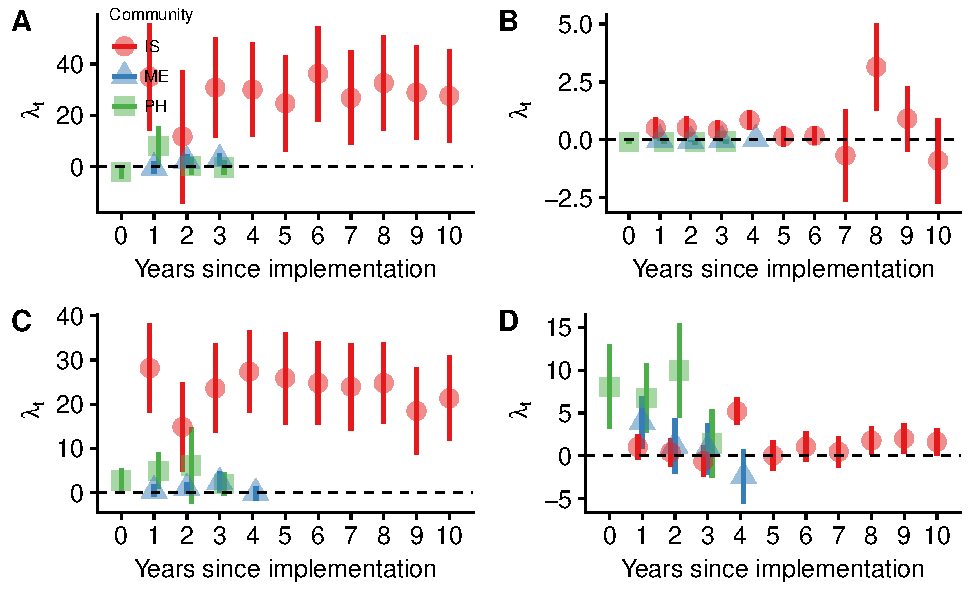
\includegraphics{Villasenor-Derbez_files/figure-latex/unnamed-chunk-5-1.pdf}
\caption{\label{fig:unnamed-chunk-5}\label{fig:indicators}Effect sizes for
marine reserves from Isla Natividad (IN; red cirlcles), Maria Elena (ME;
blue triangles), and Punta Herrero (PH; green squares) for
community-levell indicators. Plots are ordered by survey type (left:
fish; right: invertebrates) and indicators: Abundance (A, B), Richness
(C, D), Shannon's diversity index (E, F),fish biomass (G), and lobster
(\emph{Panulirus spp}) abundances (H). Points are jittered hotizontally
to avoid overplotting. Points indicate the effect size, and errorbars
are heteroskedastic-robust standard errors.}
\end{figure}

\begin{figure}
\centering
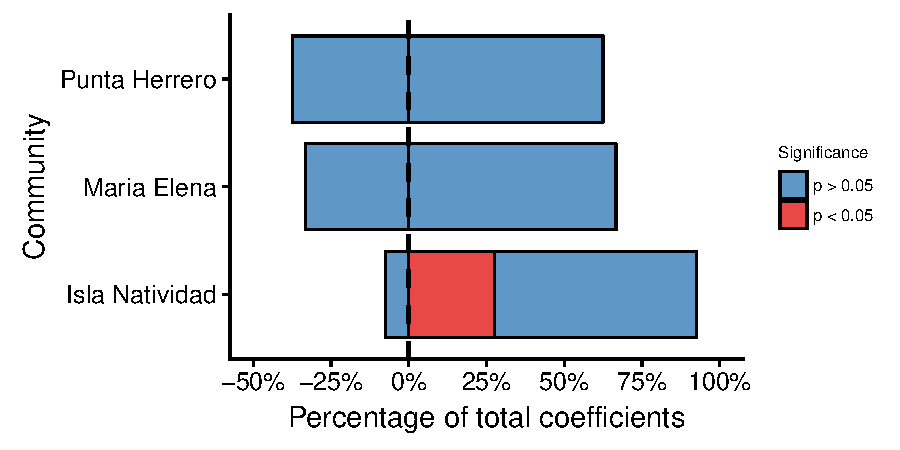
\includegraphics{Villasenor-Derbez_files/figure-latex/unnamed-chunk-6-1.pdf}
\caption{\label{fig:unnamed-chunk-6}\label{fig:res_com}Summarized effects of
the marne reserves by direction (positive - negative) and significance.}
\end{figure}

\begin{figure}
\centering
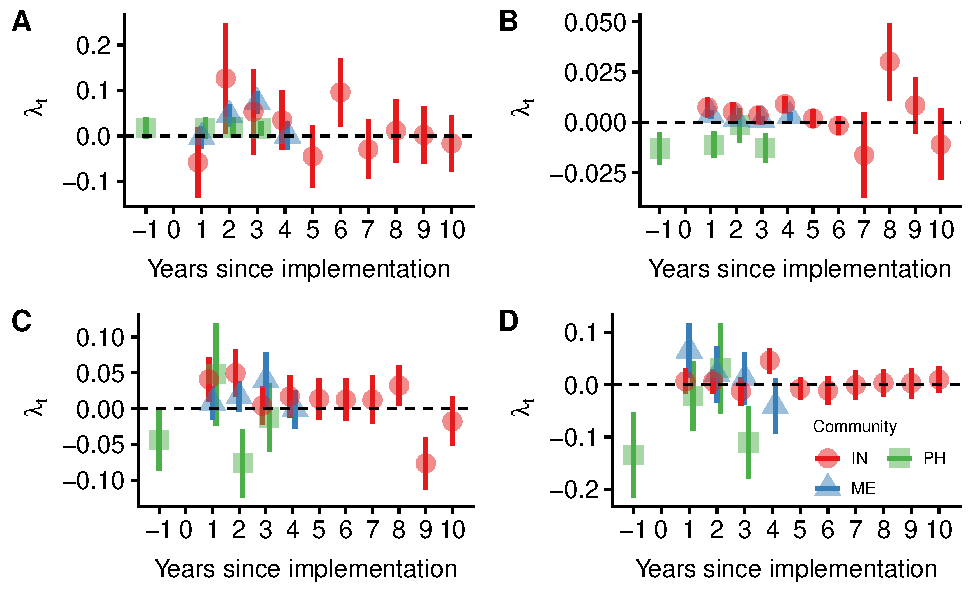
\includegraphics{Villasenor-Derbez_files/figure-latex/unnamed-chunk-8-1.pdf}
\caption{\label{fig:unnamed-chunk-8}\label{fig:lobsters}Effect sizes for
lobster catches (A) and revenues (B) in at Isla Natividad (IN; red
circles) and Maria Elena (ME; blue triangles)}
\end{figure}

\begin{table}

\caption{\label{tab:unnamed-chunk-9}\label{table:gov_res}Analysis of the fishing cooperatives based on the Social-Ecological systems framework \citep{mcginnis_2014}.}
\centering
\begin{tabular}[t]{>{\raggedright\arraybackslash}p{10em}|>{\raggedright\arraybackslash}p{10em}|l|l|l}
\hline
 & Indicator & Isla Natividad & Maria Elena & Punta Herrero\\
\hline
\textbf{Resource systems (RS)} & \textbf{} & \textbf{} & \textbf{}\\
\hline
RS2 – Clarity of system boundaries & TURF presence & High & High & High\\
\hline
RS3 – Size of resource system &  &  &  & \\
\hline
RS5 – Productivity of system & Type of ecosystem & High & High & High\\
\hline
RS7 – Predictability of system dynamics & Intensity of environmental disturbance & Low (ENSO) & High & High\\
\hline
RS9 – Location & Proximity to other communities/cities & Isolated & Not Isolated & Not Isolated\\
\hline
\textbf{Governance systems (GS)} & \textbf{} & \textbf{} & \textbf{}\\
\hline
GS1 – Government organizations & Presence of fishing cooperatives & Yes & Yes & Yes\\
\hline
GS2 – Nongovernment organizations & Involved actors & Yes & Yes & Yes\\
\hline
GS3 – Network structure & Presence of an inter-cooperative structure & Yes & No & No\\
\hline
GS4 – Property-rights systems & TURF presence & Yes & Yes & Yes\\
\hline
GS5 – Operational-choice rules & Fishing Regulations / MPA enforcement / Enforcement technolofy & Yes & Yes & Yes\\
\hline
GS6 – Collective-choice rules & Cooperative regulations & Yes & Yes & Yes\\
\hline
GS7 – Constitutional-choice rules &  &  &  & \\
\hline
\textbf{Resource units (RU)} & \textbf{} & \textbf{} & \textbf{}\\
\hline
RU1 – Resource unit mobility & Targeted species home range & Low & Medium & Medium\\
\hline
RU2 – Growth or replacement rate & Max age of targeted species & Low & Medium & Medium\\
\hline
RU4 – Economic value & Price of targeted species & high & High & high\\
\hline
\textbf{Actors (A)} & \textbf{} & \textbf{} & \textbf{}\\
\hline
A1 – Number of relevant actors &  & 98 &  & \\
\hline
A2 – Socioeconomic attributes &  &  &  & \\
\hline
A5 – Leadership/entrepreneurship & Leadership & High & High & High\\
\hline
A6 – Norms (trust-reciprocity)/social capital--- (Based on illegal fishing) & Level of illegal fishing & High & High & Low\\
\hline
A8 – Importance of resource (dependence) & Presence of alternative livelihoods & High & High & High\\
\hline
\end{tabular}
\end{table}

\clearpage

\section{Discussion}\label{discussion}

Our results show idiosyncratic biological effects of the reserves across
communities and indicators. However, many of these effects were not
statistically significant, indicating no effect of the reserve
\ref{fig:res_com}. The socioeconomic indicators pertaining to landings
and revenues associated to those landings showed little or no temporal
change before and after reserve implementation. These contrasting
effects, however, might be clarified when understanding the
social-ecological context in which these communities and their reserves
sit. In this section, we discuss potential shortcomings in our analysis,
and provide plausible explanations to the observed biological and
socioeconomic basing on previous literature and our analysis of the
social-ecological system.

The contrasting biological effectiveness observed is perhaps explained
by our approach to evaluate the temporal and spatial changes of each
indicator. Some works have solely focused on an inside-outside
comparison of indicators
\citep{guidetti_2014-8Z,friedlander_2017-oI,rodriguez_2017-PD}, which do
not address temporal variability \citep{depalma_2018}. Other works have
compared the trend observed within a reserve through time
\citep{betti_2017-lq}, which cannot distinguish between the temporal
trends in a reserve and the entire system \citep{depalma_2018}. By
accounting for trends between sites and through times, we can control
for time and space dynamics, and provide a better identification of the
effect. However, it is worth looking deeper into each case, and
identifying other plausible explanations.

Age, isolation, and enforcement are important factors influencing
effectiveness of a marine reserve \citep{edgar_2014-UO}. Isla Natividad
has the oldest reserve, is fairly isolated, and has a well-established
community-based enforcement system. While other communities are
certainly within reach, these are known to be well organized fishing
communities with successful resource management
\citep{mccay_2017-1m,mccay_2014-CN}. The reserve at Isla Natividad
presented the largest percentage of significantly positive changes in
biological indicators (19\%), but an important portion of was also
negative (15\%). With the age, relative isolation, and enforcement level
of this reserve, it would be expected for it to be considerably
effective. The potential gap in performance can be attributed to
perturbations that do not distinguish reserve boundaries, such as
environmental variability (\textbf{no recuerdo esta cita}). The region
is known to be under the influence of recurrent hypoxia and
high-temperature events known to cause massive adult mortalities
\citep{micheli_2012-EU}.

Maria Elena and Punta Herrero are relatively young reserves (See Table
\ref{table:com_sum}). From these, the Maria Elena exhibited the highest
performance in terms of biological indicators (15\% significantly
positive). In contrast, Punta Herrero had a similar proportion of
positive and negative effects.

The way in which we measure changes in catches and revenues can not
identify whether the observed differences are simply caused by
pre-existing temporal trends or by the implementation of the reserve.
Yet, there were no detectable changes in these indicators, except for
landings in Isla Natividad. Other research has shown that reserves in
Isla Natividad yield fishery benefits for the abalone fishery
\citep{rossetto_2015-V0}. Since the trend was not detected in catches
--directly related to abundance and fishing effort-- it is plausible
that these differences are purely explained by an increase in
market-level prices.

The fact that there was no detectable change in catches for Maria Elena
and Punta Herrero can be explained by a combination of factors related
to the design, management, age, or ecological factors. Reserves in these
communities are relatively small and young, and may need more time for
lobster abundances to increase enough to export larvae or adult
organisms. Other community-based marine reserves in tropical ecosystems
have taken up to six years to show a spillover effect
\citep{dasilva_2015-zX}. A complimentary explanation lies in the results
observed for the governance system. The lack of enforcement in Punta
Herrero, for example, could explain the lack of effectiveness observed
in their reserves.

\textbf{Limitations\ldots{}}

Our results show that community-based marine reserves can be effective
if the environmental and social settings allow it. By studying the
social-ecological system as a whole, we can provide a wider range of
explanations to the patterns observed. It is interesting that even under
the best enabling social conditions, climate variability can hinder the
effect of a reserve --Although it is interesting to imagine what the
state of that fishery had been if the reserve and organized cooperative
were not present--. On the contrary, we show how under low climate
variability, absence of proper governance structures can limit the
effectiveness and benefits of a reserve. Whether the combination of a
stable environment and governance structures are additive or
multiplicative represents an interesting area for future research,
especially under a changing climate.

\section*{Conflict of Interest Statement}

The authors declare that the research was conducted in the absence of
any commercial or financial relationships that could be construed as a
potential conflict of interest.

\section*{Author Contributions}

JC and EA analyzed and interpreted data, discussed the results, and
wrote the manuscript. AS, SF and JT edited the manuscript and discussed
the results.

\section*{Funding}

JCVD CONACyT + LAFF ASC SF JT

\section*{Acknowledgments}

The authors wish to acknowledge Arturo Hernández and Imelda Amador for
contributions on the governance data, as well as pre-processing
biological data. This study would have not been possible without the
effort by members of the communities here mentioned, who collected the
biological data.

\section*{Supplemental Data}

\href{http://home.frontiersin.org/about/author-guidelines#SupplementaryMaterial}{Supplementary Material}
should be uploaded separately on submission, if there are Supplementary
Figures, please include the caption in the same file as the figure.
LaTeX Supplementary Material templates can be found in the Frontiers
LaTeX folder

\paragraph*{S1 Figure}
\label{S1_Figure}

Timeseries of indicators for IN

\paragraph*{S2 Figure}
\label{S2_Figure}

Timeseries of indicators for ME

\paragraph*{S3 Figure}
\label{S3_Figure}

Timeseries of indicators for PH

\paragraph*{S1 Table}
\label{S1_Table}

Coefficient estimates for Isla Natividad

\paragraph*{S2 Table}
\label{S2_Table}

Coefficient estimates for Maria Elena

\paragraph*{S3 Table}
\label{S3_Table}

Coefficient estimates for Punta Herrero

\bibliographystyle{frontiersinSCNS_ENG_HUMS}\bibliography{references}

\section*{Figure captions}



\end{document}
